% Adapted from Template for American Journal of Undergraduate Research

\documentclass[10pt]{article}
\usepackage[explicit]{titlesec}
\setlength{\parindent}{0pt}
\setlength{\parskip}{1em}
\usepackage{hyphenat}
\usepackage{ragged2e}
\RaggedRight

% These commands change the font. If you do not have Garamond on your computer, you will need to install it.
\usepackage{garamondx}
\usepackage[T1]{fontenc}
\usepackage{amsmath, amsthm}
\usepackage{graphicx}
\usepackage{float}

% This adjusts the underline to be in keeping with word processors.
\usepackage{soul}
\setul{.6pt}{.4pt}


% The following sets margins to 1 in. on top and bottom and .75 in on left and right, and remove page numbers.
\usepackage{geometry}
\geometry{vmargin={1in,1in}, hmargin={.75in, .75in}}
\usepackage{fancyhdr}
\pagestyle{fancy}
\pagenumbering{gobble}
\renewcommand{\headrulewidth}{0.0pt}
\renewcommand{\footrulewidth}{0.0pt}

% These Commands create the label style for tables, figures and equations.
\usepackage[labelfont={footnotesize,bf} , textfont=footnotesize]{caption}
\captionsetup{labelformat=simple, labelsep=period}
\newcommand\num{\addtocounter{equation}{1}\tag{\theequation}}
\renewcommand{\theequation}{\arabic{equation}}
\makeatletter
\renewcommand\tagform@[1]{\maketag@@@ {\ignorespaces {\footnotesize{\textbf{Equation}}} #1.\unskip \@@italiccorr }}
\makeatother
\setlength{\intextsep}{10pt}
\setlength{\abovecaptionskip}{2pt}
\setlength{\belowcaptionskip}{-10pt}

\renewcommand{\textfraction}{0.10}
\renewcommand{\topfraction}{0.85}
\renewcommand{\bottomfraction}{0.85}
\renewcommand{\floatpagefraction}{0.90}

% These commands set the paragraph and line spacing
\titleformat{\section}
  {\normalfont}{\thesection}{1em}{\MakeUppercase{\textbf{#1}}}
\titlespacing\section{0pt}{0pt}{-10pt}
\titleformat{\subsection}
  {\normalfont}{\thesubsection}{1em}{\textit{#1}}
\titlespacing\subsection{0pt}{0pt}{-8pt}
\renewcommand{\baselinestretch}{1.15}

% This designs the title display style for the maketitle command
\makeatletter
\newcommand\sixteen{\@setfontsize\sixteen{17pt}{6}}
\renewcommand{\maketitle}{\bgroup\setlength{\parindent}{0pt}
\begin{flushleft}
\sixteen\bfseries \@title
\medskip
\end{flushleft}
\textit{\@author}
\egroup}
\makeatother

% This styles the bibliography and citations.
%\usepackage[biblabel]{cite}
\usepackage[sort&compress]{natbib}
\setlength\bibindent{2em}
\makeatletter
\renewcommand\@biblabel[1]{\textbf{#1.}\hfill}
\makeatother
\renewcommand{\citenumfont}[1]{\textbf{#1}}
\bibpunct{}{}{,~}{s}{,}{,}
\setlength{\bibsep}{0pt plus 0.3ex}





\title{Local Network Audit and Exploration with Nmap}

\author{
Larsen Close \\ \medskip 
Computer Science, Metropolitan State University, Denver, CO \\ 
Student: lclose@msudenver.edu \\
}

\pagestyle{empty}
\begin{document}

% Makes the title and author information appear.
\vspace*{.01 in}
\maketitle
\vspace{.12 in}

\section*{abstract}
Extensive Nmap scanning is used to fingerprint a local network with clear instruction given for replication and key areas of interest are identified. 
Anomalies, security concerns and unexpected results are discussed and further pursued. A detailed account of supplemental tools used and actions prompted by 
 the findings is given before presenting conclusions and a reflection.

\section*{motivation}
We often only pay attention to our internet connected devices when we lose connectivity. We then try and restore the connection as quickly
as possible. As the Internet Of Things expands and our world increasingly digitizes so does the danger to our privacy, security and 
safety. These devices warrant attention, as believing someone else is protecting our privacy, security and safety is negligently naive. 
The steps clearly demonstrated in this paper are steps we should all take regularly for our own sake and for the sake of our loved ones.
\vspace{.12 in}

\section*{introduction}

I started fingerprinting my network with a few areas of heightened interest. In order to ensure a thorough investigation I first used widespread scanning and looked for abnormalities, 
anything which surprised me or that raised security concerns. I made sure to turn on and log into every device on the network before conducting the scans. Also in order to asses the behavior 
of a new automated system for the door lock and thermostat(mandated by the property owner) I connected this device to the network for the first time. The device has been running on cellular  
but has an ethernet option as well. 

\subsection*{how does Tails handle local traffic?}

I was curious about the local network scan response of Tails, The Amnesic Incognito Live System (a security-focused Debian based distribution of Linux) so I booted a machine 
with the live system before the scans. Starting with cursory scans and increasing the intensity each time while saving results created a detailed fingerprint 
of the network.

\subsection*{let shodan.io scan for you}

To check on the networks public IP address and look for any outward facing access I used shodan.io.\cite{shodan}
After using their search function I created a monitor with triggers to notify me of any any unexpected activity. After scanning extensively I created the table below to organize
my findings, visualize them and decide where to increase focus. Host data from the scans was combined with DHCP Reservations from the routers then supplemented with previous knowledge 
where applicable.

\section*{methods and measurement}
To begin we need to know which IP addresses to scan. Using the command: \begin{verbatim}ifconfig | grep broadcast\end{verbatim} 
We can determine the local networks and the subnet ranges. As seen in \textbf{Figure \ref{ifconfig image}}, the networks are \verb|10.0.0.0/24|
and \verb|192.168.0.0/24|. The \verb|netmask 0xffffff00| tells us the range for hosts is limited the last octet, digits 1-254.

\begin{figure}[H]
\centering
\includegraphics[width=0.5\textwidth]{images/ifconfig.png}
\caption{First the command 'ifconfig | grep broadcast' identifies the local networks.}\label{ifconfig image}
\end{figure}

\subsection*{rivileges for scanning}
Next a ping scan  quickly lists the hosts. It's likely that you will not get a full list if you do not run this command with super user privileges.
Testing without sudo resulted in 1 host and 9 hosts. To ping scan both networks:
\begin{verbatim}
sudo nmap -sn 192.168.0.0/24
sudo nmap -sn 10.0.0.0/24 
\end{verbatim}

\begin{figure}[H]
\centering
\includegraphics[width=0.4\textwidth]{images/ping.png}
\caption{Ping scans returning 14 and 7 hosts.}\label{ping image}
\end{figure}
As we can see in \textbf{Figure \ref{ping image}}, the ping scan with sudo returned a list of 14 hosts and 7 hosts respectively. 

\subsection*{flags for more thorough scans}
After completing the ping scan, using nmap with the flag \verb|-A| will initiate an aggressive scan. Including \verb|-v| increases the 
verbosity of the results and \verb|-T5| turns the speed all the way up. The commands used:
\begin{verbatim}
sudo nmap -T5 -A -v 192.168.0.0/24
sudo nmap -T5 -A -v 10.0.0.0/24\end{verbatim}
At this point it was necessary to create \textbf{Table \ref{local table}} to organize results and create an overview that could be visualized. The more thorough
scans return so much information that it demands systematic organization. Zenmap can do a good job of helping with this but it has not been running
well for me on macOS Catalina. Another option which I employed is to use an additional flag when running nmap, \verb|-oX 'scan-%T-%D.xml'| which outputs the
scan in xml format named by the date and time. For example:
\begin{verbatim}
sudo nmap -oX 'scan-%T-%D.xml' -T5 -A -v 192.168.0.0/24
sudo nmap -oX 'scan-%T-%D.xml' -T5 -A -v 10.0.0.0/24\end{verbatim}

\subsection*{monitoring IP addresses with shodan.io}
Due to the ethical and legal restrictions on scanning the public IP owned by Century Link I used shodan.io to search and set up a monitor for the address.\cite{shodan}
An easy what to determine your public IP address is:
\begin{verbatim}
curl ifconfig.me
\end{verbatim}

\section*{results}
Shodan.io allowed us to determine that the router has an open outward facing port running http with authentication on 4567.\cite{shodan} \textbf{Figure \ref{shodan image}} 
shows a screen shot from their web service.

\begin{figure}[H]
\centering
\includegraphics[width=0.5\textwidth]{images/shodan.png}
\caption{From website https://www.shodan.io/ often called "the most dangerous search engine in the world"}\label{shodan image}
\end{figure}

\subsection*{compiling results}
The table below, \textbf{Table \ref{local table}}, is a compilation of all the scans. The aggressive scans discovered more hosts missed by the ping scans.
Immediately some interesting things are visible from the table. My HomePod has two IP addresses on the same network. After logging into and checking the router
it appears both are running on the same 5G WiFi network. While going through the results I was familiar with everything except for host 192.168.0.32 which was running ssh
on port 22. I checked the routers DCHP Reservations and found no information there either. Scans showed the mac address \verb|80:1F:12:C6:CF:77| as well as some
additional information. Seen here using a targeted aggressive scan of just this device: \verb|sudo nmap -T5 -A 192.168.0.32| 

\begin{figure}[H]
\centering
\includegraphics[width=0.5\textwidth]{images/unknown.png}
\caption{Resulting scan of unfamiliar device}\label{unknown image}
\end{figure}

\begin{table}[H]
  \begin{center}
  \begin{tabular}{ | c | c | c | c | c | c | c | c | } 
  \hline
   & \textbf{Hostname} & \textbf{Device} & \textbf{Purpose} & \textbf{OS} & \textbf{Open} & \textbf{Filtered}  & \textbf{Services}  \\  
   \hline
   \textbf{10.0.0.1} & Dionysus & Router & Gateway & Linux & 53,80,443,10000 & - & ssl,http \\  
   \hline
   \textbf{10.0.0.29}  & HD100 & Webcam & Security & - & 554,49152 & - & rtsp,UPnP \\  
   \hline
   \textbf{10.0.0.77}  & Daemon & HomePod & Music & audioOS & 62078 & 24 dif & wiretap\\  
   \hline
   \textbf{10.0.0.80}  & Veritas & MacLaptop & PC & macOS & 3000 & - & grafana \\  
   \hline
   \textbf{10.0.0.97}  & Daemon & HomePod & Music & audioOS & 6 dif & 100 dif & wiretap \\  
   \hline
   \textbf{10.0.0.124}  & Mercury & Watch & Fit & watchOS & - & 17 dif & wiretap/track \\  
   \hline
   \textbf{10.0.0.155}  & raspberrypi & rpi & dev & Buster & 22 & - & ssh \\  
   \hline
   \textbf{}  &  &  &   &  &  &  & \\  
   \hline
   \textbf{192.168.0.1}  & Century Link & Router & Gateway & Linux & 23,80,433,8085 & - & telnet\\  
   \hline
   \textbf{192.168.0.2}  & Dionysus & Router & Secondary & Linux & All & - & - \\  
   \hline
   \textbf{192.168.0.3}  & raspberrypi & rpi & dev & Buster & 22 & - & ssh \\  
   \hline
   \textbf{192.168.0.4}  & DESKTOP.. & WindowsPC & PC & Windows & - & All & - \\  
   \hline
   \textbf{192.168.0.31} & Veritas & MacLaptop & PC & macOS & 3000 & - & grafana \\
   \hline
   \textbf{192.168.0.32} & Unknown & ? & 80:1f:12:c6:cf:77 & Linux & 22 & - & ssh \\
   \hline
   \textbf{192.168.0.33} & Unknown & HPLaptop & tails & tails live & - & All & - \\  
   \hline
   \textbf{192.168.0.100}  & Ares & rpi & motion & Buster & 22,3389,8081 & - & xrdp,motion \\  
   \hline
   \textbf{192.168.0.101}  & Master & rpi & Kubernetes & Buster & 22,80,443 & - & - \\  
   \hline
   \textbf{192.168.0.102}  & Node1 & rpi & Kubernetes & Buster & 22,80,443 & - & - \\  
   \hline
   \textbf{192.168.0.103}  & Node2 & rpi & Kubernetes & Buster & 22,80,443 & - & - \\  
   \hline
   \textbf{192.168.0.104}  & Node3 & rpi & Kubernetes & Buster & 22,80,443 & - & - \\  
   \hline
   \textbf{192.168.0.105}  & Node4 & rpi & Kubernetes & Buster & 22,80,443 & - & - \\  
   \hline
   \textbf{192.168.0.106}  & Node5 & rpi & Kubernetes & Buster & 22,80,443 & - & - \\  
   \hline
  \end{tabular}
  \caption{Compilation of the results from all scans. Purpose column filled from previous knowledge of the network.}
  \label{local table}
  \end{center}
  \end{table}

\subsection*{identifying the unknown device}
Attempting to connect via ssh to the device confirmed that it was not something I was familiar with. I change all of my ssh
connections to passwordless key based authentication. Which is more secure than the password based authentication
running on this device which allowed me to connect and try passwords as well as connect as root to try passwords which 
I regularly disallow. Rather than attempting to brute force the password I followed the mac address.

\subsection*{researching the OUI}
Nmap includes a lookup of the mac addresses OUI, organizationally unique identifier, the first three octets.
\begin{verbatim}
MAC Address: 80:1F:12:C6:CF:77 (Microchip Technology)
\end{verbatim}

\subsection*{binary note}
\begin{verbatim}
  In the decimal notation representing the last octet of our networking addresses 3 digits are 
  required whereas here hexadecimal notation is used and only two digits are required. Both of 
  these represent 8 binary digits and have 256 unique possibilities. Usually indexed at 0 so 
  0-255 and in the case of networking some addresses are reserved, such as broadcast on 255.
\end{verbatim}

The products section of Microchip Technologies website at \verb|https://www.microchip.com/| includes embedded architecture,
security, smart monitoring and networking devices among others.\cite{microchip} This prompted the question, could my smart device
for the lock on my door have started running a password based ssh connection on my network as soon as I plugged in the 
ethernet cable?

\subsection*{yes - unplug that device}
Immediately unplugging the device then rescanning confirmed this hypothesis, see \textbf{Figure \ref{down image}}.

\begin{figure}[H]
\centering
\includegraphics[width=0.5\textwidth]{images/down.png}
\caption{Rescan after unplugging}\label{down image}
\end{figure}




\section*{conclusions}
The foregoing results prompted further action. To look more closely into \verb|port 4567| running \verb|tram| open to the entire internet I enabled telnet to
explore the device. I was curious to see if the port could be closed but did not find a method. Important to note here that telnet can usually be easily enabled by 
logging into your routers admin page at its IP address in a browser. Do not forget to disable telnet after finishing with it. While researching Century Links C2100T router 
I did find an ADSL attack vector using nmap listed:\cite{techni}
\begin{verbatim}
nmap -sS -sV -vv -n -Pn -T5 A.B.C.D -p80 -oG -
\end{verbatim}
The attack was summarized - \verb|using nmap to look for an open port 80 on a huge block of IP addresses|.\cite{techni}
However, I found nothing related nor any further information on exploit-db or google. I did find a generally related 
article, \verb|The weakest link on the network: exploiting ADSL routers to perform cyber-attacks|, published by the IEEE 
in 2013 discussing the authors discovery of two 0-day vulnerabilities and expounding upon the vulnerabilities of ADSL routers.\cite{journal} Of course my conscience of the ethical 
and legal concerns prevented me from attempting any thing like this myself without explicit permission.

\subsection*{not-so smart devices}
The most concerning finding was the smart device which controls my lock and was mandated for every unit in the building. Along with a possible network attack vector, 
I was able to plug and unplug the device because it is not stored in a secure cabinet. All of the devices in my building are the same so if one is compromised 
every unit is compromised. Likely nationwide a huge number of homes would be compromised. Here in \textbf{Figure \ref{fcc image}} are the FCC IDs for the device.
\begin{figure}[H]
\centering
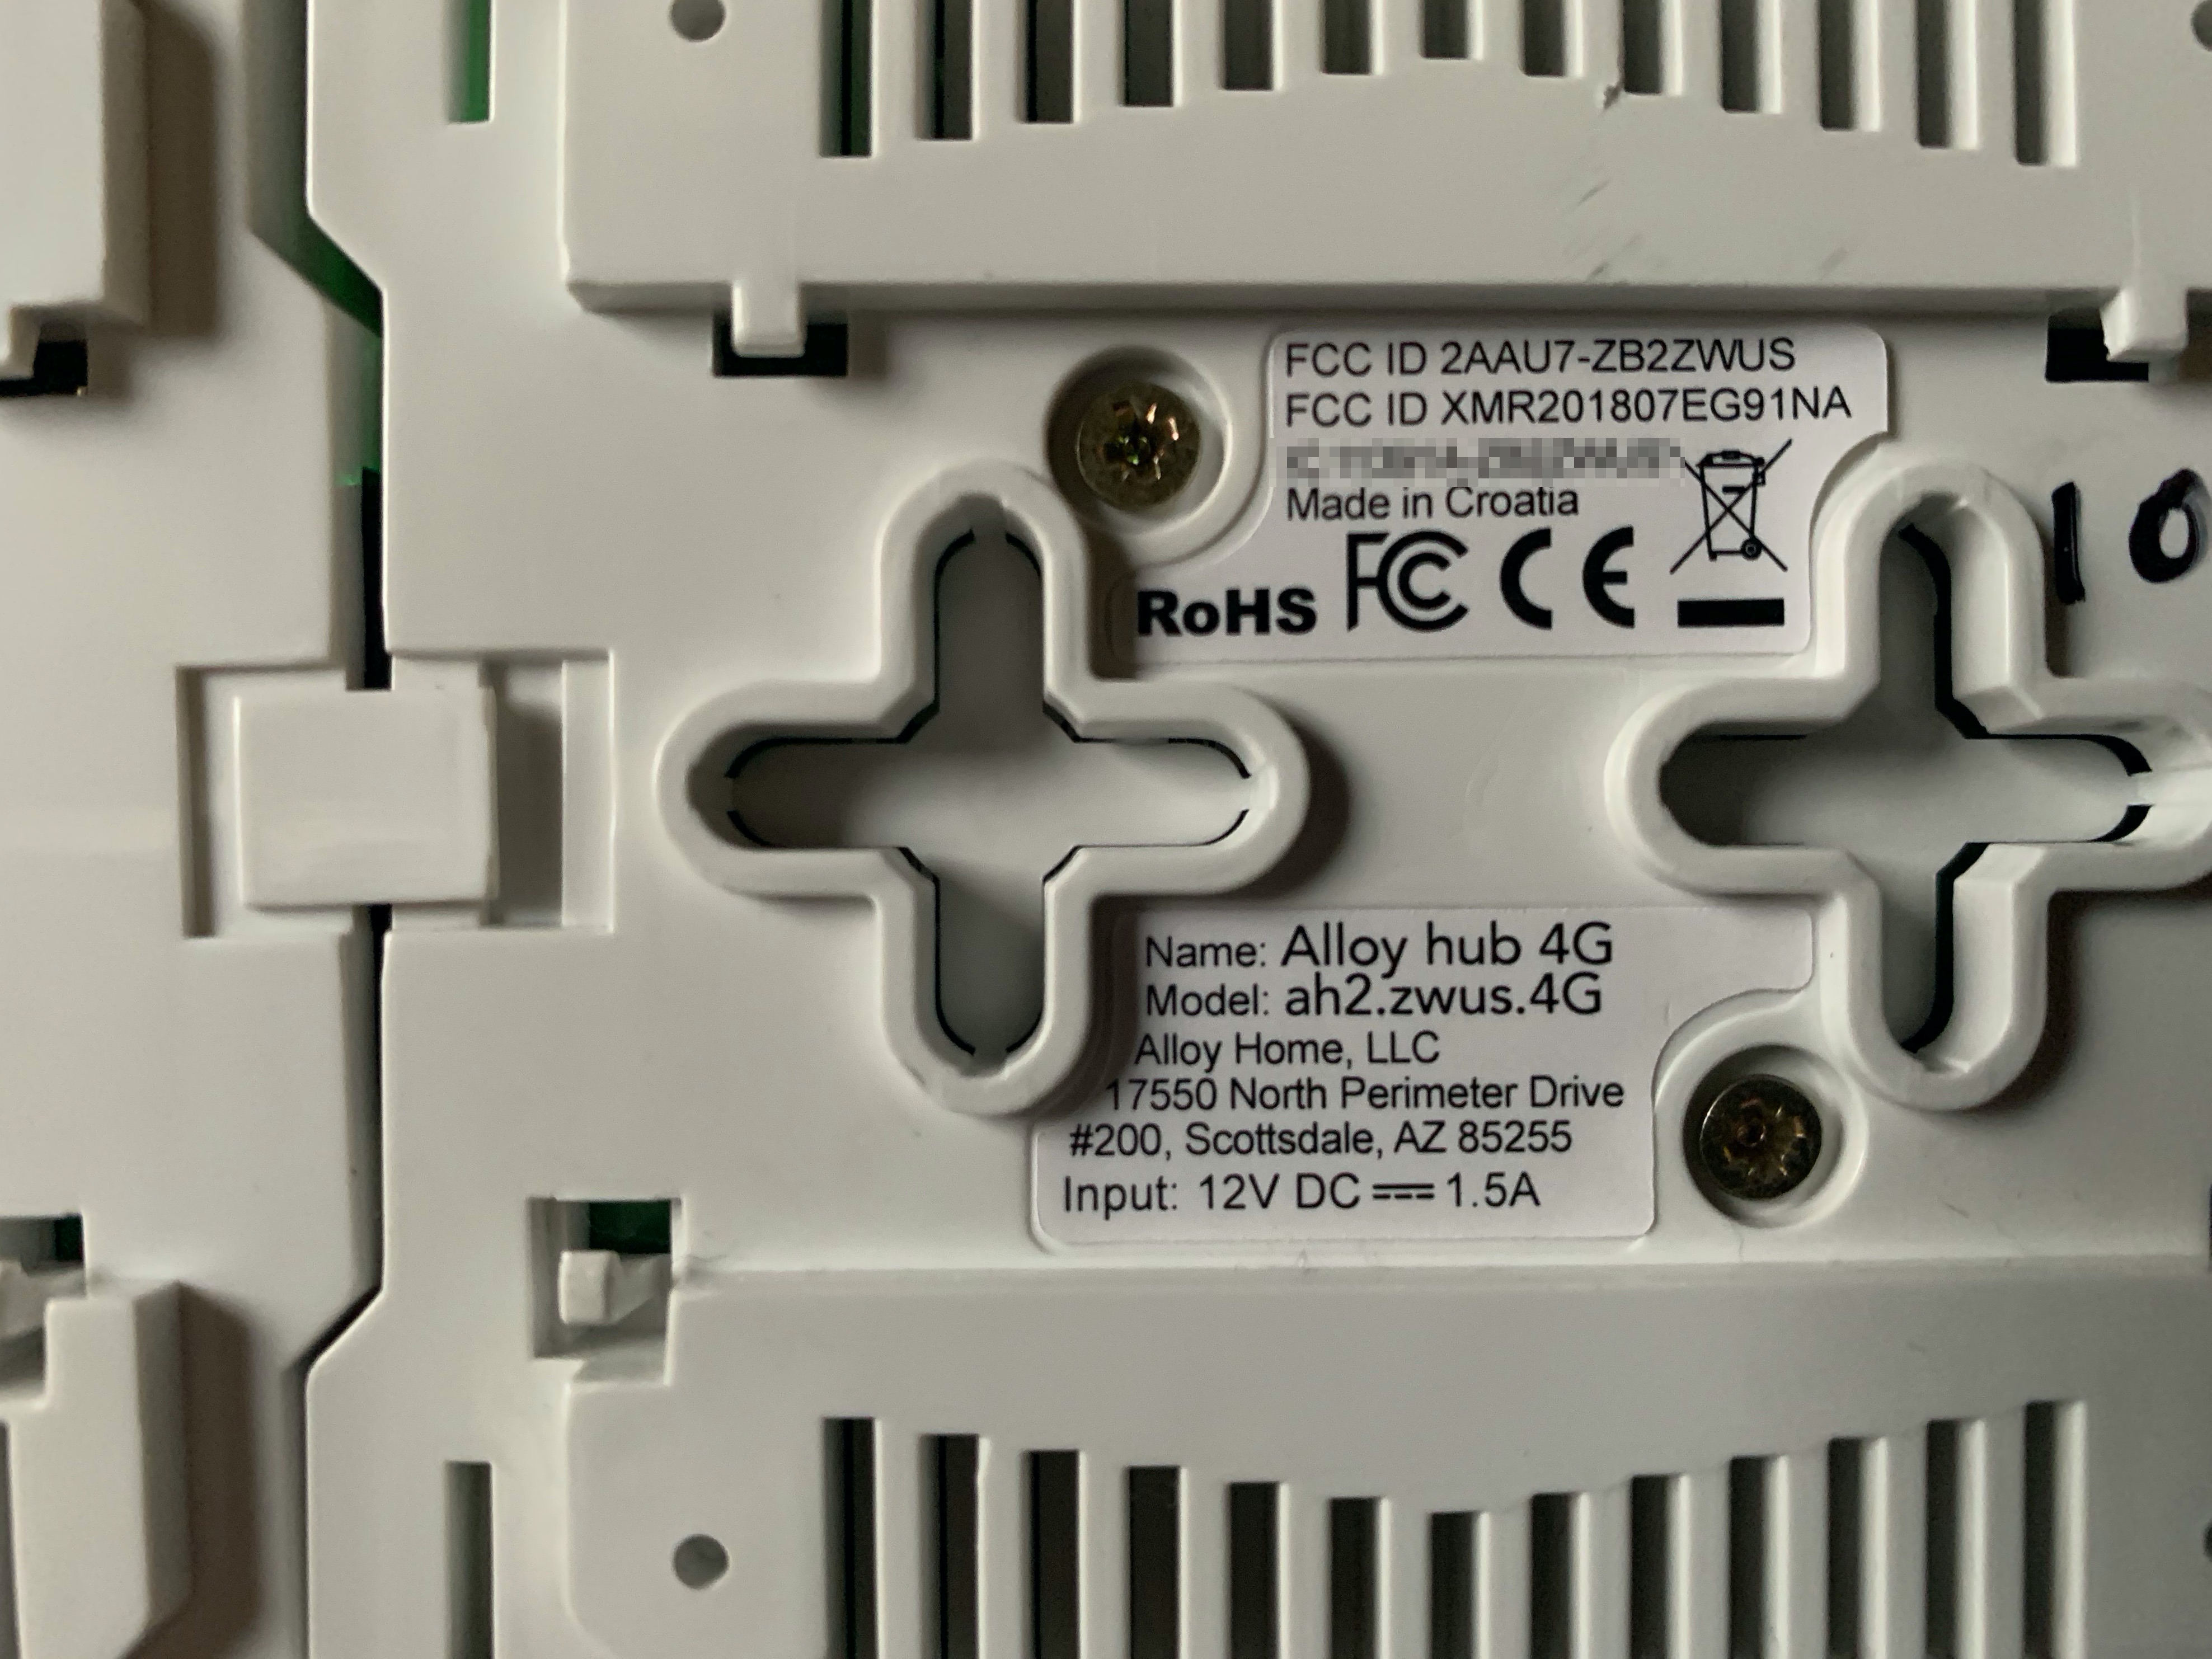
\includegraphics[width=0.5\textwidth]{images/fcc.png}
\caption{The FCC ID's clearly displayed}\label{fcc image}
\end{figure}

\subsection*{fcc id}
The FCC ID's are \verb|2AAU7-ZB2ZWUS XMR201807EG91NA| the records for which are all public. The FCC website is pretty terrible to use but using
\verb|www.fcc.io| we can search the FCC site using a much better UI. The records tell us the device has a Quectel Wireless chip for the cellular connection, with a list of
the frequencies, and a Z-Wave module for the radio connection to the lock.\cite{fcc} The records give us two possible frequencies for the Z-wave. One of which is shown in
\textbf{Figure \ref{radio image}}. It is beyond the scope of this paper but a software defined radio could be used to capture and analyze the signals on that frequency.

\begin{figure}[H]
\centering
\includegraphics[width=0.5\textwidth]{images/radio.png}
\caption{Radio frequency}\label{radio image}
\end{figure}

\subsection*{nmap OS fingerprinting}
Many of the devices on the network have unrecognized operating systems, for these cases nmap asks we submit the fingerprint if the OS is known. I tried to submit 
fingerprints but ran into a bug on the site. There is no section on the submission form for writing what the OS actually is, \textbf{Figure \ref{bug image}}. 
Alternatively the unknown services submission site has the section missing from the OS submission form. I signed up to the dev-mailing list, as suggested by the site for bug 
reporting, and will try and see if the bug is known.\cite{submit} I also ran into several issues with Zenmap on Catalina, issues installing, running, saving scans and crashing
when selecting topology.

\medskip

\subsection*{next steps}
In addition to continuing research on the network and hosts, next steps include more testing on these issues and bug reporting to nmap dev-list and issue
trackers.

\begin{figure}[H]
\centering
\includegraphics[width=0.95\textwidth]{images/bug.png}
\caption{Nmap OS fingerprint submission page missing OS name category}\label{bug image}
\end{figure}

\begin{thebibliography}{9} 

\bibitem{journal} Stasinopoulos, Ntantogian and  Xenakis(2013) The weakest link on the network: Exploiting ADSL routers to perform cyber-attacks, \textit{IEEE International Symposium on Signal Processing and Information Technology} 000135-000139. \textit {https://doi.org/10.1109/ISSPIT.2013.6781868}

\bibitem{shodan} The search engine for The Internet of Things, \textit{https://www.shodan.io/} (accessed June 2020)

\bibitem{techni} Technicolor C2100T, \textit{https://charlesreid1.com/wiki/Technicolor\_C2100T} (accessed June 2020)

\bibitem{microchip} Microchip Technology Inc, \textit{https://www.microchip.com/} (accessed June 2020)

\bibitem{fcc} Federal Communications Commission, \textit{https://www.fcc.gov/} (accessed June 2020)

\bibitem{submit} Nmap Fingerprint Submitter, \textit{https://nmap.org/cgi-bin/submit.cgi?new-os} (accessed June 2020)

\end{thebibliography}


\section*{reflection}
Throughout this exploration there was constant learning, experienced gained and improvement of my network configuration. I realized that I should be turning 
grafana off when I am not using it until I have it setup with production level security. I decided that my smart device was better off 
having less connectivity and that I would not be plugging it into my local network. With more time I would have looked more closely into exactly
what was and wasn't returned from the different nmap scans including UDP scans and see if I could find more information locally using options for 
firewall and IDS evasion. The questions I brought to the paper were all answered and I was left with new questions replacing them.

\subsection*{tails}
I found out what is returned from tails during network scans, nothing at all and a mac address which automatically changes on every boot.
I had heard that the issue of what to do with local network traffic on tails had still not been completely resolved but I take it that is mostly
referring to what the machine running tails wants to do on the local network.

\subsection*{surprises}
It was astounding to see how many services actively run on my HomePod and my appleWatch. Also strange to learn that my HomePod is using two
IP addresses. I used the UncOver zero-day on iOS a couple weeks ago to jailbreak an old iPad. My hope was to find something like Little Snitch
for iOS but regardless it's nice to have root access to my iPad and be able to ssh to it. Maybe an approach like this would work for the HomePod to
monitor in real time just what is actually happening with all those services.

\subsection*{telnet}
I hadn't ever explored the telnet connection to my CenturyLink device. It was interesting to see how different the telnet interfaces are between devices. 
I found methods for closing the open 4567 port running tram on other manufacturers routers but almost none of the commands were consistent or even available 
between devices.

\subsection*{z-wave}
I'd been meaning to research the smart device and so I was glad to get an excuse to spend some time doing so. I've read the current version of Z-wave is 
relatively secure but found some talk about downgrade attacks forcing devices to use older versions. I have some other Z-wave devices here so I'm curious
to see if I can get them to connect. I have a HackRF-One software defined radio and would love to do security research on Z-wave but time is always a limiting 
factor as well as the strict and tricky legality concerns, especially when dealing with radio. I did find a 2020 paper using the HackRF-One to do denial of service
attacks on Z-wave versions s0-s2 but haven't seen much beyond that.

\subsection*{latex}
I also used this as an opportunity use LaTeX for the first time, which I borderline came to regret as I realized there was some learning curve. I especially 
struggled towards the end figuring out formatting for the bibliography and citations while tired and needing to finish. Which I am still not certain are exactly
but are on track with the guidelines and their clarity. Using LaTeX probably more than most else led to the paper taking significant time but also added to what 
was learned and gave incredible control in formatting.
\end{document}
